%
%\addtocontents{toc}{\newpage}
\chapter{Principal Component Analysis}
\label{cpt:pca}

Principal Component Analysis (PCA) is a powerful tool for 

\section{The PCA method}

Given a matrix $M$, we can use a linear algebra technique called singular value decomposition (SVD) to solve for matrices $U, S, V$ such that $M = U * S * V^T.$  For a given $k$ number of components


\begin{figure}[ht]
	\centering
	\subfigure[]{
		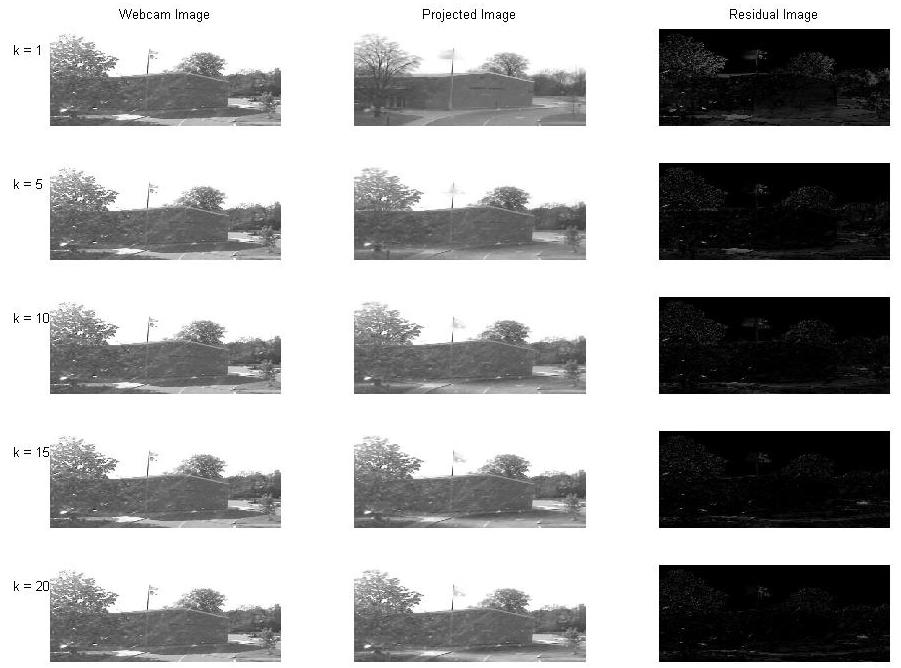
\includegraphics[width=1\textwidth]{figures/pcaIntroFigs.jpg}
	\label{fig:pcaIntroFigs}
	}
	\subfigure[]{
		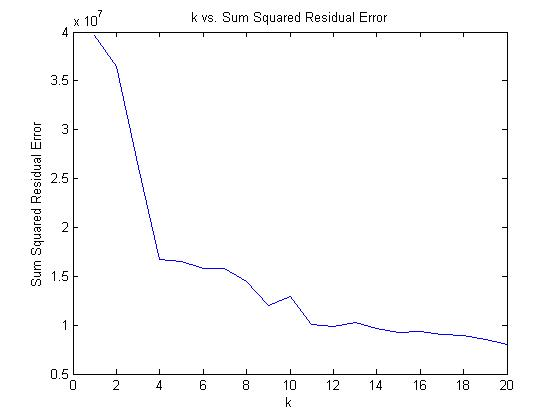
\includegraphics[width=.8\textwidth]{figures/pcaIntroPlot.jpg}
	\label{fig:pcaIntroPlot}
	}
		\caption[Learning a sky mask for a webcam scene.]{Figure \ref{fig:pcaIntroFigs} shows the first PCA component of a webcam scene.  By adding or subtracting this component, we control how dark or how light the sky is. Figure \ref{fig:pcaIntroPlot} shows that a simple thresholding of this image effectively segments the sky from the rest of the image.}
\end{figure}

\subsection{Incremental PCA}

In situations where dataset sizes conflict with memory constraints, we can use a modified algorithm called Incremental PCA.  Incremental PCA [reference to Matthew Brand]